\chapter{Applicazione di SFA: La Tramvia di Firenze}
In questo capitolo verr\`a analizzata una particolare applicazione di un KF al problema del posizionamento ferrotramviario.\\*
Nell'ambito di un progetto di ricerca finanziato dall'Unione Europea, si \`e voluto studiare l'usabilit\`a di KF come sistema di posizionamento ferrotramviario alternativo a quello descritto nel Capitolo 1, il quale fa un largo uso di apparati installati a terra, fatto che si vorrebbe minimizzare.\\*
La linea ferrotramviaria scelta come ambiente di prova \`e la linea \texttt{T1} della Tramvia di Firenze, che collega la stazione di \emph{Villa Costanza}, sita nel comune di Scandicci all'altezza dell'omonimo parcheggio di interscambio dell'autostrada \texttt{A1}, all'ospedale di \emph{Careggi}, sito quest'ultimo nel comune di Firenze.
\begin{figure}[h]
	\centering
	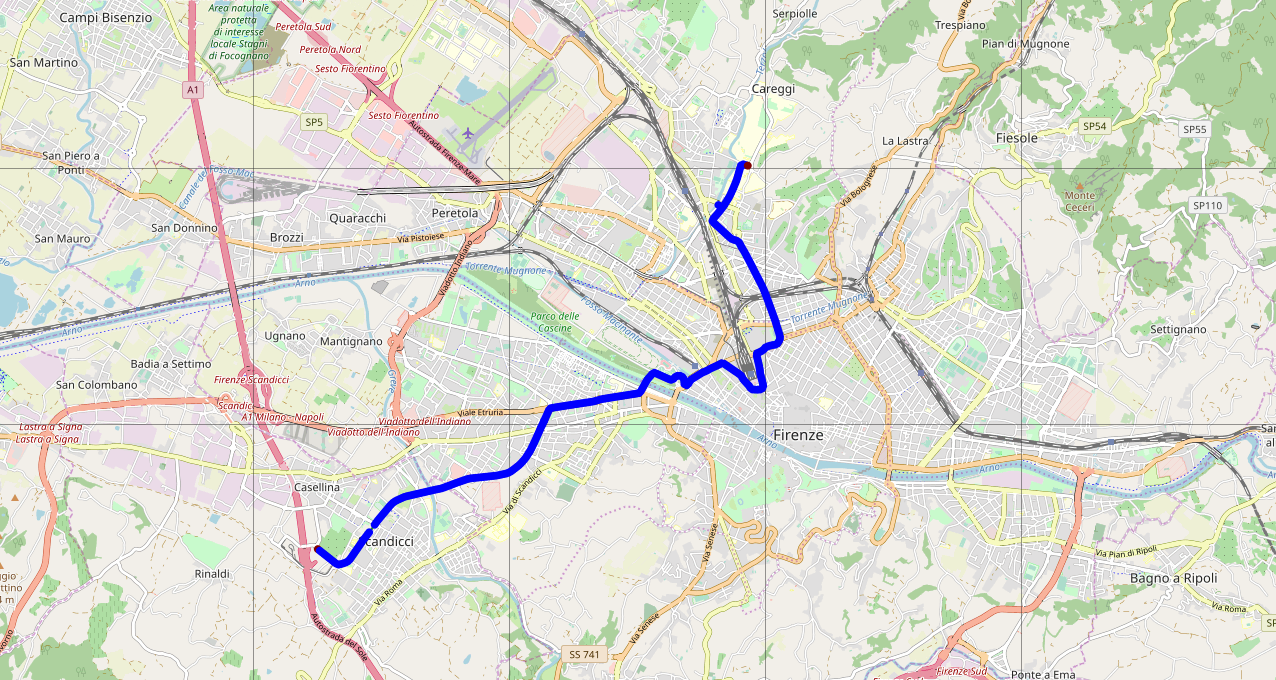
\includegraphics[width=\linewidth]{img/t1}
	\caption{Tramvia di Firenze - Linea \texttt{T1}}
	\label{fig:t1}
\end{figure}
\section{Architettura di Sistema}
Il sistema progettato ha lo scopo di eseguire SFA su una piattaforma hardware \texttt{Nvidia TX-Jetson} installata bordo treno, la quale riceve i dati \emph{raw} dai sensori e li elabora al fine di stimare la progressiva chilometrica del treno in ciascun istante di tempo.\\*
Tale posizione sar\`a inviata, attraverso un modem \texttt{LTE}:
\begin{itemize}
	\item All'OBCU, per essere utilizzata attivamente all'interno del sistema di \emph{interlocking}
	\item Ad un arbitario host che esegue un software grafico di tracciamento del treno: il \texttt{RailTrackTool} (RTT)
\end{itemize}
\subsection{Architettura lato treno}
Sul treno \`e stata installata una scheda 